\documentclass[aspectratio=169]{beamer}

% -------------------------
% 1.  PACKAGES & THEME
% -------------------------
\usepackage[english]{babel}
\usepackage{fontawesome5}
\usepackage{tikz}
\usetikzlibrary{positioning,calc,shapes.geometric,backgrounds,patterns}
\usepackage{FiraSans}
\usepackage{FiraMono}
\usepackage{graphicx}
\usepackage{hyperref}
\usepackage{booktabs}s
\usepackage{pgf-pie}
\usepackage{xcolor}

% Theme & colors
\usetheme{metropolis}
\definecolor{monero}{HTML}{FF6600}
\definecolor{solana}{HTML}{9945FF}
\definecolor{meteora}{HTML}{00D1FF}
\definecolor{darkbg}{HTML}{0B0F1A}
\definecolor{midbg}{HTML}{1A1F2E}
\definecolor{lightaccent}{HTML}{2D3748}
\definecolor{fg}{HTML}{F7FAFC}
\definecolor{gold}{HTML}{FFD700}
\definecolor{neon}{HTML}{00FFFF}
\definecolor{brightpurple}{HTML}{9945FF}

\setbeamercolor{background canvas}{bg=darkbg}
\setbeamercolor{normal text}{fg=fg}
\setbeamercolor{alerted text}{fg=monero}
\setbeamercolor{example text}{fg=solana}
\setbeamercolor{frametitle}{fg=fg,bg=darkbg}
\setbeamercolor{title}{fg=fg}

\setbeamerfont{title}{size=\Huge,series=\bfseries}
\setbeamerfont{subtitle}{size=\Large}
\setbeamerfont{author}{size=\normalsize}
\setbeamerfont{date}{size=\small}
\setbeamerfont{frametitle}{size=\Large,series=\bfseries}

% No nav symbols, clean footer with slide numbers
\setbeamertemplate{navigation symbols}{}
\setbeamertemplate{footline}{%
  \hfill%
  \usebeamerfont{page number in head/foot}%
  \color{fg!60}\insertframenumber\,/\,\inserttotalframenumber\kern1em\vskip2pt%
}

% Custom itemize bullets
\setbeamertemplate{itemize items}[circle]
\setbeamercolor{itemize item}{fg=monero}
\setbeamercolor{itemize subitem}{fg=solana}

% -------------------------
% 2.  TITLE SLIDE
% -------------------------
\title{FUN GERBIL}
\subtitle{Fully Homomorphic Encryption}
\author{Mads Christensen × Kyle Koshiyama × Eric Nans}
\date{Q3 2025}

\begin{document}

% -------------------------------------------------
\begin{frame}[plain]
  
\begin{tikzpicture}[remember picture,overlay]
    % Epic gradient background with overlays
    \fill[darkbg] (current page.south west) rectangle (current page.north east);
    \fill[monero,opacity=0.15] (current page.south west) -- 
          (current page.north west) -- 
          ([yshift=-3cm]current page.north east) -- 
          ([yshift=2cm]current page.south east) -- cycle;
    \fill[solana,opacity=0.1] ([xshift=3cm]current page.south west) -- 
          ([xshift=-2cm]current page.north west) -- 
          (current page.north east) -- 
          (current page.south east) -- cycle;
    
    % Animated circuit pattern overlay
    \foreach \x in {0,1,2,...,20} {
      \foreach \y in {0,1,2,...,12} {
        \fill[neon,opacity=0.03] ([shift={(0.8*\x cm, 0.8*\y cm)}]current page.south west) circle (0.5pt);
      }
    }
    
    % Main title content with epic styling
    \node[align=center] at (current page.center){
      % Main title - MASSIVE and bold with glow effect
      {\fontsize{72}{80}\selectfont\color{neon!40}\textbf{FUN GERBIL}}\\[-4.6em]
      {\fontsize{72}{80}\selectfont\color{white}\textbf{FUN GERBIL}}\\[1.2em]
      
      % Subtitle - clean and simple
      {\fontsize{42}{50}\selectfont\color{monero}\textbf{onboarding Monero}}
    };
    
    % Corner decorative elements
    \fill[gold,opacity=0.8] (current page.south west) -- ++(2,0) -- ++(0,0.1) -- ++(-2,0) -- cycle;
    \fill[meteora,opacity=0.8] (current page.north east) -- ++(-2,0) -- ++(0,-0.1) -- ++(2,0) -- cycle;
    
  \end{tikzpicture}
\end{frame}

% -------------------------------------------------
\begin{frame}[t]{\color{brightpurple}\textbf{The Problem: Two Ecosystems, Two Challenges}}

  \vspace{0.5em}
  
  \begin{columns}[T]
    % Left column - Solana Problems
    \begin{column}{0.48\textwidth}
      \centering
      \begin{tikzpicture}
        % Background box for Solana
        \fill[solana,opacity=0.15,rounded corners=15pt] (-3.5,-4.2) rectangle (3.5,2.2);
        
        % Solana Logo
        \node at (0,1.5) {\includegraphics[height=1.2cm]{solana-logo.png}};
        
        % Title
        \node[text=solana,font=\Large\bfseries] at (0,0.5) {\textcolor{solana}{Solana}};
        
        % Three problems
        \node[text=monero,font=\large,drop shadow={shadow xshift=0.05cm,shadow yshift=-0.05cm,opacity=0.3}] at (-2.5,-0.7) {\faEye};
        \node[text=fg,font=\normalsize\bfseries,align=left,text width=4.5cm] at (0.3,-0.7) {Public Account\\Balances};
        
        \node[text=gold,font=\large,drop shadow={shadow xshift=0.05cm,shadow yshift=-0.05cm,opacity=0.3}] at (-2.5,-1.9) {\faUserSecret};
        \node[text=fg,font=\normalsize\bfseries,align=left,text width=4.5cm] at (0.3,-1.9) {Every Transaction\\Visible};
        
        \node[text=neon,font=\large,drop shadow={shadow xshift=0.05cm,shadow yshift=-0.05cm,opacity=0.3}] at (-2.5,-3.1) {\faThumbsDown};
        \node[text=fg,font=\normalsize\bfseries,align=left,text width=4.5cm] at (0.3,-3.1) {Front-Running\\Attacks};
      \end{tikzpicture}
    \end{column}
    
    % Right column - Monero Problems
    \begin{column}{0.48\textwidth}
      \centering
      \begin{tikzpicture}
        % Background box for Monero
        \fill[monero,opacity=0.15,rounded corners=15pt] (-3.5,-4.2) rectangle (3.5,2.2);
        
        % Monero Logo
        \node at (0,1.5) {\includegraphics[height=1.2cm]{monero-logo.png}};
        
        % Title
        \node[text=monero,font=\Large\bfseries] at (0,0.5) {\textcolor{monero}{Monero}};
        
        % Two problems
        \node[text=gold,font=\large,drop shadow={shadow xshift=0.05cm,shadow yshift=-0.05cm,opacity=0.3}] at (-2.5,-1.3) {\faCode};
        \node[text=fg,font=\normalsize\bfseries,align=left,text width=4.5cm] at (0.3,-1.3) {No Native Smart\\Contracts or Scripting};
        
        \node[text=neon,font=\large,drop shadow={shadow xshift=0.05cm,shadow yshift=-0.05cm,opacity=0.3}] at (-2.5,-2.8) {\faBan};
        \node[text=fg,font=\normalsize\bfseries,align=left,text width=4.5cm] at (0.3,-2.8) {Facing Exchange\\Delistings};
      \end{tikzpicture}
    \end{column}
  \end{columns}

\end{frame}

% -------------------------------------------------
\begin{frame}{\color{brightpurple}\textbf{Fun Gerbil: Products}}
  \begin{tikzpicture}[remember picture,overlay]
    \fill[gold,opacity=0.05] (current page.south west) rectangle (current page.north east);
  \end{tikzpicture}

  \centering

  \begin{tikzpicture}
    % Three square product boxes
    
    % Atomic Swaps
    \fill[monero,opacity=0.15,rounded corners=12pt] (-6.8,0) rectangle (-2.6,4.2);
    \node[text=monero,font=\Huge,drop shadow={shadow xshift=0.15cm,shadow yshift=-0.15cm,opacity=0.4}] at (-4.7,3) {\faRandom};
    \node[text=white,font=\huge\bfseries,align=center] at (-4.7,1.5) {Atomic\\Swaps};
    
    % Wrapped Monero
    \fill[solana,opacity=0.15,rounded corners=12pt] (-2.1,0) rectangle (2.1,4.2);
    \node[text=solana,font=\Huge,drop shadow={shadow xshift=0.15cm,shadow yshift=-0.15cm,opacity=0.4}] at (0,3) {\faCube};
    \node[text=white,font=\huge\bfseries,align=center] at (0,1.5) {Wrapped\\Monero};
    
    % Fully Homomorphic Encryption
    \fill[meteora,opacity=0.15,rounded corners=12pt] (2.6,0) rectangle (6.8,4.2);
    \node[text=meteora,font=\Huge,drop shadow={shadow xshift=0.15cm,shadow yshift=-0.15cm,opacity=0.4}] at (4.7,3) {\faLock};
    \node[text=white,font=\huge\bfseries,align=center] at (4.7,1.5) {ZK\\FHE};
  \end{tikzpicture}
  
\end{frame}

% -------------------------------------------------
\begin{frame}{\color{brightpurple}\textbf{Comprehensive Privacy Solutions}}
  \begin{tikzpicture}[remember picture,overlay]
    \fill[monero,opacity=0.05] (current page.south west) rectangle (current page.north east);
  \end{tikzpicture}
  
  \centering
  \vspace{2em}
  \begin{tikzpicture}
    % Two prominent partner logo boxes with clipped images
    
    % DarkLake logo box
    \node[rounded corners=15pt, minimum width=5cm, minimum height=5cm, 
          draw=fg!40, line width=2pt, fill=midbg, fill opacity=0.8,
          path picture={
            \clip[rounded corners=15pt] (path picture bounding box.south west) rectangle (path picture bounding box.north east);
            \node at (path picture bounding box.center) {
              \includegraphics[width=4.8cm,height=4.8cm,keepaspectratio]{darklake.jpeg}
            };
          }] at (-3.5,2.5) {};
    
    % Arcium logo box
    \node[rounded corners=15pt, minimum width=5cm, minimum height=5cm,
          draw=fg!40, line width=2pt, fill=midbg, fill opacity=0.8,
          path picture={
            \clip[rounded corners=15pt] (path picture bounding box.south west) rectangle (path picture bounding box.north east);
            \node at (path picture bounding box.center) {
              \includegraphics[width=4.8cm,height=4.8cm,keepaspectratio]{arcium.jpg}
            };
          }] at (3.5,2.5) {};
  \end{tikzpicture}
  
\end{frame}

% -------------------------------------------------
\begin{frame}{\color{brightpurple}\textbf{Live Demo}}
  \begin{tikzpicture}[remember picture,overlay]
    \fill[monero,opacity=0.05] (current page.south west) rectangle (current page.north east);
  \end{tikzpicture}
  
  % Two column layout
  \begin{columns}[c]
    % Left column for text
    \begin{column}{0.45\textwidth}
      \centering
      
      % Title
      {\LARGE\color{gold}\textbf{FUN GERBIL SWAP TERMINAL}}
      
      {\normalsize\color{meteora}Live demo: \textbf{fungerbil.com}}
      
    \end{column}
    
    % Right column for image
    \begin{column}{0.55\textwidth}
      \centering
      \includegraphics[height=0.75\textheight,width=\textwidth,keepaspectratio]{ui.png}
    \end{column}
  \end{columns}
  
\end{frame}

% -------------------------------------------------
\begin{frame}[t]{\color{brightpurple}\textbf{Business Model}}
  \begin{tikzpicture}[remember picture,overlay]
    \fill[monero,opacity=0.05] (current page.south west) rectangle (current page.north east);
  \end{tikzpicture}
  
  \centering
  \vspace{1.5em}
  
  \begin{tikzpicture}
    % Revenue streams in clean boxes
    \fill[monero,opacity=0.15,rounded corners=10pt] (-7,2) rectangle (-2.5,4.5);
    \node[text=monero,font=\Large] at (-4.75,3.8) {\faPercentage};
    \node[text=white,font=\large\bfseries,align=center] at (-4.75,3.1) {0.08\%};
    \node[text=fg!80,font=\normalsize,align=center] at (-4.75,2.5) {Swap Fee};
    
    \fill[meteora,opacity=0.15,rounded corners=10pt] (-2,2) rectangle (2,4.5);
    \node[text=meteora,font=\Large] at (0,3.8) {\faCoins};
    \node[text=white,font=\large\bfseries,align=center] at (0,3.1) {0.03\%};
    \node[text=fg!80,font=\normalsize,align=center] at (0,2.5) {Liquidity Fee};
    
    \fill[gold,opacity=0.15,rounded corners=10pt] (2.5,2) rectangle (7,4.5);
    \node[text=gold,font=\Large] at (4.75,3.8) {\faClock};
    \node[text=white,font=\large\bfseries,align=center] at (4.75,3.1) {E-TWAP, Limit Orders};
    \node[text=fg!80,font=\normalsize,align=center] at (4.75,2.5) {Novel DeFi Primitives};
    
    % Target revenue
    \node[text=gold,font=\LARGE\bfseries] at (0,0.8) {\$100K Daily Revenue Target};
    \node[text=meteora,font=\normalsize] at (0,0.1) {.1\% of \$100M Monero daily volume};
  \end{tikzpicture}
\end{frame}

% -------------------------------------------------
\begin{frame}[t]{\color{brightpurple}\textbf{Fun Gerbil: Competitive Advantage}}
  \begin{tikzpicture}[remember picture,overlay]
    \fill[monero,opacity=0.05] (current page.south west) rectangle (current page.north east);
  \end{tikzpicture}
  
  \centering

  \begin{tikzpicture}
    % Advantage 1 - Monero's Anonymity Set
    \fill[monero,opacity=0.2,rounded corners=15pt] (-7,2.2) rectangle (7,3.4);
    \node[text=monero,font=\Large] at (-6,2.8) {\faUsers};
    \node[text=white,font=\Large\bfseries,align=left,anchor=west] at (-5.2,2.8) {Established Anonymity Set};
    
    % Advantage 2 - Open FHE and ZK Infrastructure
    \fill[solana,opacity=0.2,rounded corners=15pt] (-7,0.9) rectangle (7,2.0);
    \node[text=neon,font=\Large] at (-6,1.45) {\faLock};
    \node[text=white,font=\Large\bfseries,align=left,anchor=west] at (-5.2,1.45) {Open FHE and ZK Infrastructure};
    
    % Advantage 3 - Cross-Chain vs Intrachain
    \fill[meteora,opacity=0.2,rounded corners=15pt] (-7,-0.4) rectangle (7,0.7);
    \node[text=gold,font=\Large] at (-6,0.15) {\faLink};
    \node[text=white,font=\Large\bfseries,align=left,anchor=west] at (-5.2,0.15) {Cross-Chain, Not Intrachain};
    
    % Advantage 4 - Arcium Confidential Tokens
    \fill[brightpurple,opacity=0.2,rounded corners=15pt] (-7,-1.7) rectangle (7,-0.6);
    \node[text=meteora,font=\Large] at (-6,-1.15) {\faCoins};
    \node[text=white,font=\Large\bfseries,align=left,anchor=west] at (-5.2,-1.15) {Arcium Confidential Tokens};
  \end{tikzpicture}
\end{frame}

% -------------------------------------------------
\begin{frame}[t]{\color{brightpurple}\textbf{Market Opportunity}}
  \begin{tikzpicture}[remember picture,overlay]
    \fill[monero,opacity=0.05] (current page.south west) rectangle (current page.north east);
  \end{tikzpicture}
  
  \centering
  \vspace{2em}
  
  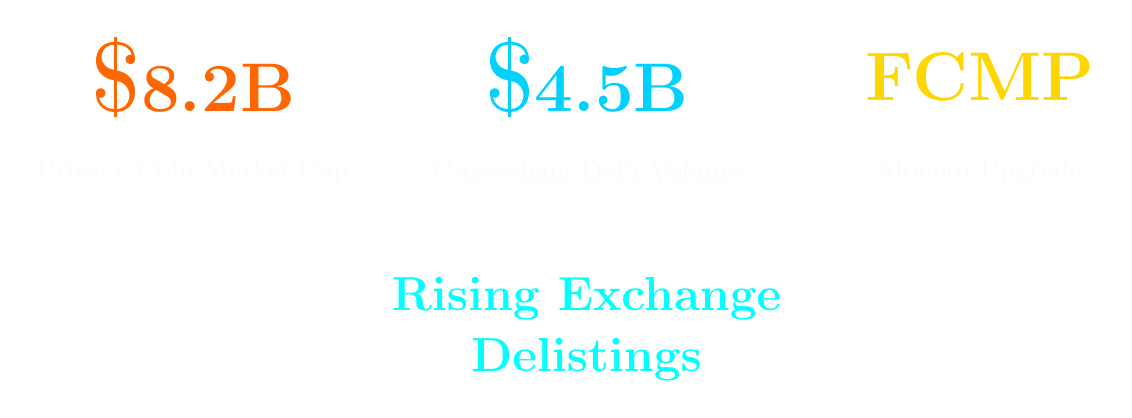
\begin{tikzpicture}
    % Four key figures - large and prominent
    
    % $8.2B
    \node[text=monero,font=\fontsize{42}{50}\selectfont\bfseries] at (-5,2) {\$8.2B};
    \node[text=fg!70,font=\normalsize] at (-5,0.8) {Privacy Coin Market Cap};
    
    % $45B
    \node[text=meteora,font=\fontsize{42}{50}\selectfont\bfseries] at (0,2) {\$4.5B};
    \node[text=fg!70,font=\normalsize] at (0,0.8) {Cross-chain DeFi Volume};
    
    % FCMP
    \node[text=gold,font=\fontsize{42}{50}\selectfont\bfseries] at (5,2) {FCMP};
    \node[text=fg!70,font=\normalsize] at (5,0.8) {Monero Upgrade};
    
    % Rising Delistings
    \node[text=neon,font=\LARGE\bfseries,align=center] at (0,-1.2) {Rising Exchange\\Delistings};
  \end{tikzpicture}
\end{frame}

% -------------------------------------------------
\begin{frame}[t]{\color{brightpurple}\textbf{Roadmap}}
  \begin{tikzpicture}[remember picture,overlay]
    \fill[monero,opacity=0.05] (current page.south west) rectangle (current page.north east);
  \end{tikzpicture}
  
  \centering
  \vspace{1em}
  
  \begin{tikzpicture}
    % Q4 2025
    \fill[monero,opacity=0.15,rounded corners=10pt] (-7.5,3) rectangle (-4.3,5.5);
    \node[text=monero,font=\Large\bfseries] at (-5.9,5) {Q4 2025};
    \node[text=white,font=\normalsize,align=center] at (-5.9,4.3) {Testnet Launch};
    \node[text=fg!70,font=\small,align=center] at (-5.9,3.7) {XMR/SOL Swaps};
    \node[text=fg!70,font=\small] at (-5.9,3.3) {\faRocket};
    
    % Q1 2026
    \fill[solana,opacity=0.15,rounded corners=10pt] (-4,3) rectangle (-0.8,5.5);
    \node[text=solana,font=\Large\bfseries] at (-2.4,5) {Q1 2026};
    \node[text=white,font=\normalsize,align=center] at (-2.4,4.3) {Mainnet};
    \node[text=fg!70,font=\small,align=center] at (-2.4,3.7) {Multi-asset};
    \node[text=fg!70,font=\small] at (-2.4,3.3) {\faCoins};
    
    % Q2 2026
    \fill[meteora,opacity=0.15,rounded corners=10pt] (-0.5,3) rectangle (2.7,5.5);
    \node[text=meteora,font=\Large\bfseries] at (1.1,5) {Q2 2026};
    \node[text=white,font=\normalsize,align=center] at (1.1,4.3) {API/SDK};
    \node[text=fg!70,font=\small,align=center] at (1.1,3.7) {TWAP Orders};
    \node[text=fg!70,font=\small] at (1.1,3.3) {\faClock};
    
    % Q3 2026
    \fill[gold,opacity=0.15,rounded corners=10pt] (3,3) rectangle (6.2,5.5);
    \node[text=gold,font=\Large\bfseries] at (4.6,5) {Q3 2026};
    \node[text=white,font=\normalsize,align=center] at (4.6,4.3) {Full Protocol};
    \node[text=fg!70,font=\small,align=center] at (4.6,3.7) {DAO Governance};
    \node[text=fg!70,font=\small] at (4.6,3.3) {\faGlobe};
    
    % Timeline arrow
    \draw[->,line width=3pt,fg!30] (-7,2.3) -- (5.7,2.3);
    \node[text=fg!60,font=\normalsize] at (-0.65,1.7) {Progressive Decentralization};
  \end{tikzpicture}
\end{frame}

% -------------------------------------------------
\begin{frame}{\color{brightpurple}\textbf{Team}}
  \begin{tikzpicture}[remember picture,overlay]
    \fill[darkbg] (current page.south west) rectangle (current page.north east);
    \fill[gold,opacity=0.1] (current page.south west) ellipse (10cm and 8cm);
  \end{tikzpicture}
  
  \centering
  \vspace{-0.5em}
  
  \begin{tikzpicture}
    % Team display moved up more
    \fill[midbg,rounded corners=20pt] (-7,-1.5) rectangle (7,3.5);
    
    \node[text=gold,font=\Large\bfseries] at (0,2.9) {FOUNDING TEAM};
    
    % Team member boxes - better sizing
    \fill[monero,opacity=0.3,rounded corners=8pt] (-6.5,0.8) rectangle (-2.2,2.3);
    \node[text=white,font=\bfseries,align=center] at (-4.35,1.9) {Mads Christensen};
    \node[text=white,font=\small,align=center] at (-4.35,1.6) {CEO \& Founder};
    \node[text=monero,font=\scriptsize,align=center] at (-4.35,1.1) {DeFi and Infrastructure\\Engineer};
    
    \fill[meteora,opacity=0.3,rounded corners=8pt] (-1.8,0.8) rectangle (1.8,2.3);
    \node[text=white,font=\bfseries,align=center] at (0,1.9) {Kyle Koshiyama};
    \node[text=white,font=\small,align=center] at (0,1.6) {FHE Engineer};
    \node[text=meteora,font=\scriptsize,align=center] at (0,1.1) {Former Fhenix\\Current DarkLake};
    
    \fill[solana,opacity=0.3,rounded corners=8pt] (2.2,0.8) rectangle (6.5,2.3);
    \node[text=white,font=\bfseries,align=center] at (4.35,1.9) {Tiago Alves};
    \node[text=white,font=\small,align=center] at (4.35,1.6) {Cryptography & ZK Expert};
    \node[text=solana,font=\scriptsize,align=center] at (4.35,1.1) {Current DarkLake};
    
    % Backing info
    \node[text=gold,font=\large,align=center] at (0,0.1) {\textbf{Fundraising}};
    \node[text=white,font=\normalsize,align=center] at (0,-0.5) {Seeking seed capital once permissionless protocols launch};
    \node[text=meteora,font=\normalsize,align=center] at (0,-1.1) {Target: \$1M seed round for protocol development};
  \end{tikzpicture}
\end{frame}

% -------------------------------------------------
\begin{frame}[standout]
  
\begin{tikzpicture}[remember picture,overlay]
    \fill[darkbg] (current page.south west) rectangle (current page.north east);
    \fill[monero,opacity=0.2] (current page.south west) -- 
          (current page.north west) -- 
          (current page.north east) -- 
          ([yshift=-4cm]current page.south east) -- cycle;
    \fill[gold,opacity=0.15] ([yshift=4cm]current page.south west) -- 
          (current page.south east) -- 
          (current page.north east) -- cycle;
          
    % Animated background elements
    \foreach \i in {1,...,30} {
      \fill[neon,opacity=0.05] (rnd*16-8, rnd*10-5) circle (rnd*0.3+0.1);
    }
  \end{tikzpicture}
  
  \centering
  \vspace{0.5em}
  
  {\fontsize{42}{50}\selectfont\color{white}\textbf{Join the}}\\
  {\fontsize{52}{60}\selectfont\color{gold}\textbf{PRIVACY}}\\
  {\fontsize{42}{50}\selectfont\color{white}\textbf{Revolution}}
  
  \vspace{1.8em}
  \begin{tikzpicture}
    \node[text=meteora,font=\Large,drop shadow] at (0,1.2) {\faGithub \quad github.com/madschristensen99/fungerbil};
    \node[text=gold,font=\Large,drop shadow] at (0,0.4) {\faTelegram \quad t.me/fungerbilswap};
    \node[text=neon,font=\Large,drop shadow] at (0,-0.4) {\faGlobe \quad fungerbil.com};
    
  \end{tikzpicture}
  
\end{frame}

\end{document}

